% override specific chktex warnings

% chktex-file 1 - ignore commands followed by a space, e.g. \\ new line here
% chktex-file 3 - enclose previous parentheses wit {}
% chktex-file 9 - sometimes messes up with ( and {
% chktex-file 36 - put a space in front of parentheses
% chktex-file 45 - don't use $$ instead of \[, etc
% chktex-file 46 - don't use $ instead of \(, etc

\documentclass[10pt, onesided]{amsart}
% \usepackage[showboxes]{textpos}

\usepackage[absolute,overlay]{textpos}
\setlength{\TPHorizModule}{1.0cm}
\setlength{\TPVertModule}{\TPHorizModule}
\textblockorigin{0.0cm}{0.0cm}  %start all at upper left corner

\usepackage{amsmath}
\usepackage{amsthm}
\usepackage{amsfonts}
\usepackage{amssymb}
\usepackage{mathpazo}
\usepackage{booktabs}
\usepackage[usenames,x11names]{xcolor}
\usepackage{tikz}
\usepackage{textcomp}
\usepackage[letterpaper]{geometry}
\geometry{verbose,tmargin=0.5in,bmargin=0.5in,lmargin=0.75in,rmargin=0.5in}
\usepackage{multicol}
\usepackage{bm}
\usepackage{comment}
\usepackage{cancel}
\usepackage{array}
\usepackage{gensymb}
\usepackage{enumerate}

\usepackage[many]{tcolorbox}

\pagestyle{plain}
\raggedright
\renewcommand{\familydefault}{\sfdefault}
\setlength{\parskip}{\medskipamount}
\setlength{\columnsep}{1cm}

\everymath{\displaystyle}
\setlength{\parskip}{\bigskipamount}

% counter for resuming enumerated list numbers
\newcounter{resumeenumi}
\newcommand{\suspend}{\setcounter{resumeenumi}{\theenumi}}
\newcommand{\resume}{\setcounter{enumi}{\theresumeenumi}}

\newcommand\lb{\linebreak}
\newcommand\pars{\par\smallskip}
\newcommand\parm{\par\medskip}
\newcommand\parb{\par\bigskip}

\makeatletter
\providecommand{\gettikzxy}[3]{%
	\tikz@scan@one@point\pgfutil@firstofone#1\relax
	\edef#2{\the\pgf@x}%
	\edef#3{\the\pgf@y}%
}
\makeatother



% full width colored block but color specifiable
%\cb[body bg strength]{header bg}{header text}{body text}
\newcommand{\cb}[4][15]{
	\setbeamercolor{block title}{bg = #2}
	\setbeamercolor{block body}{bg = #2!#1}
	\setbeamercolor{item projected}{bg=#2, fg=white}
	\begin{center}
		\begin{block}{#3}
			#4
		\end{block}
	\end{center}
}

% colored block with width specified
% \cbw[body bg strength]{header bg}{width}{header text}{body text}
\newcommand{\cbw}[5][15]{
	\begin{center}
		%\vspace{-0.35cm}
		\begin{minipage}{#3\textwidth}
			\setbeamercolor{block title}{bg= #2}
			\setbeamercolor{block body}{bg= #2!#1}
			\setbeamercolor{item projected}{bg=#2, fg=white}
			\begin{block}{#4}
				\raggedright
				#5
			\end{block}
		\end{minipage}
	\end{center}
}

% centered minipage with text \raggedright
%\cmini[width]{content}
\newcommand{\cmini}[2][0.8]{
	\begin{center}
		\begin{minipage}{#1\columnwidth}
			\raggedright
			#2
		\end{minipage}
	\end{center}
}

%left flushed minipage
\newcommand{\mini}[2][0.8]{
	\begin{minipage}{#1\columnwidth}
		\raggedright
		#2
	\end{minipage}
}

%left flushed minipage, top aligned
\newcommand{\minit}[2][0.8]{
	\begin{minipage}[t]{#1\columnwidth}
		\raggedright
		#2
	\end{minipage}
}

%left flushed minipage
% \newcommand{\miniT}[2][0.8]{
%  \begin{minipage}[T]{#1\columnwidth}
%   \raggedright
%   #2
%  \end{minipage}
% }

%left flushed minipage
\newcommand{\minib}[2][0.8]{
	\begin{minipage}[b]{#1\columnwidth}
		\raggedright
		#2
	\end{minipage}
}

\newcommand{\cfig}[2][1]{% centred, scaled graphic
	\begin{center}
		\includegraphics[scale=#1]{#2}
	\end{center}
}
% figure with tight border for photos
% \cfigb[saitMaroon]{borderwidth with unit}{scale}{image}
\newcommand{\cfigb}[4][structure]{
	% \usepackage{adjustbox}
	\setlength{\fboxrule}{1pt}
	\begin{center}
		\includegraphics[scale=#3, cframe= #1 #2]{#4}
	\end{center}
}

\newcommand{\imgbox}[3]{
	% \setlength{\fboxsep}{12pt}
	\includegraphics[scale=#1, cframe= structure #3]{#2}
}

% \imgboxbg[bg color=white]{scale}{path/to/img}{border color}{border, e.g. 2pt}{margin, e.g. 4pt}
\newcommand{\imgboxbg}[6][white]{
	\setlength{\fboxrule}{#5}
	\setlength{\fboxsep}{#6}
	\centering
	\fcolorbox{#4}{#1}{\includegraphics[scale=#2]{#3}}
}

\newcommand{\fig}[2][1]{% scaled graphic
	\includegraphics[scale=#1]{#2}
}

% centred framed  box black border
%\cbox[width]{content}
\newcommand{\cbox}[2][0.9]{% framed centered  box
	\setlength\fboxsep{0.042\columnwidth}
	\setlength\fboxrule{0.0015\columnwidth}
	\begin{center}
		\fcolorbox{black}{white}{
			\vspace{-0.5cm}
			\begin{minipage}{#1\columnwidth}
				\raggedright
				#2
			\end{minipage}
		}
	\end{center}
	\setlength\fboxsep{0cm}
}



\newtcolorbox{mybox}[1][]
{
	colback=white,
	top=0.25cm,
	bottom=0.25cm,
	left=0.25cm,
	right=0.25cm,
	colframe=structure,
	fonttitle=\bfseries,
	enhanced, drop fuzzy shadow,
	% attach boxed title to top left={yshift=-2mm, xshift=5mm},
	attach boxed title to top left={yshift=-2mm, xshift=5mm}, colbacktitle=structure!80!white, #1}

\newtcolorbox{plainbox}[1][]{colback=white, sharp corners, top=0.125cm, bottom=0.125cm, left=0pt, right=0pt, boxrule=0.5pt,colframe=structure,fonttitle=\bfseries, colbacktitle=structure, arc=0mm, #1}
%
\newtcbtheorem{myexam}{Example}%
{
	enhanced,
	colback=white,
	top=0.375cm,
	bottom=0.25cm,
	left=0.375cm,
	right=0.375cm,
	colframe=structure,
	fonttitle=\bfseries,
	drop fuzzy shadow,
	%description font=\mdseries\itshape,
	attach boxed title to top left={yshift=-2mm, xshift=5mm},
	colbacktitle=structure!80!white
	}{exam}% then \pageref{exer:theoexample} references the theo

\newcommand{\myexample}[2][red]{
	% \tcb\tcbset{theostyle/.style={colframe=red,colbacktitle=yellow}}
	\begin{myexam}{}{}
		\raggedright
		#2
	\end{myexam}
	% \tcbset{colframe=structure,colbacktitle=structure}
}

\newtcbtheorem{myexer}{Exercise}%
{
	enhanced,
	colback=white,
	top=0.375cm,
	bottom=0.25cm,
	left=0.375cm,
	right=0.375cm,
	colframe=structure,
	fonttitle=\bfseries,
	drop fuzzy shadow,
	%description font=\mdseries\itshape,
	attach boxed title to top left={yshift=-2mm, xshift=5mm},
	colbacktitle=structure!80!white
	}{exer}

\newcommand{\myexercise}[2][red]{
	% \tcb\tcbset{theostyle/.style={colframe=red,colbacktitle=yellow}}
	\begin{myexer}{}{}
		\raggedright
		#2
	\end{myexer}
	% \tcbset{colframe=structure,colbacktitle=structure}
}


\begin{document}

\thispagestyle{empty}
\vspace{-7cm}
\centering


\textbf{\Large Module 5: Friction Losses (CIVL 318)}
\par\medskip
\begin{center}
	\begin{tabular}{r >{$}r<{$} >{$}c<{$} >{$}l<{$}}
		\toprule
		\addlinespace
		\textbf{ Reynolds Number}:  & N_R               & =           & \frac{vD\rho}{\eta}                     \\
		\addlinespace
		                            & N_R < 2000        & \Rightarrow & \text{laminar}                          \\
		\addlinespace
		                            & 2000 < N_R < 4000 & \Rightarrow & \text{critical flow}                    \\
		
		\addlinespace
		                            & N_R > 4000        & \Rightarrow & \text{turbulent flow}                   \\
		\addlinespace
		\midrule
		\addlinespace
		\textbf{Laminar flow:}      & f                 & =           & \frac{64}{N_R}                          \\
		\addlinespace
		\midrule
		\addlinespace
		\textbf{Turbulent flow:}:   & f                 & =           &                                         
		\frac{0.25}{\left[\log\left(\frac{1}{3.7\left(D/\epsilon\right)}+\frac{5.74}{N_R^{0.9}}\right)\right]^2}  \\
		\addlinespace
		\midrule
		\addlinespace
		\textbf{ Darcy's Equation}: & h_L               & =           & f\times \frac{L}{D}\times\frac{v^2}{2g} \\
		\addlinespace
		\bottomrule
	\end{tabular}
	
	\vspace{2cm}
	
	\begin{center}
		\textbf{Roughness, $\epsilon$}:
		\par\bigskip
		\begin{tabular}{rrl}
			\toprule
			Material (new, clean)          & $\qquad$ & $\epsilon$ (m)     \\
			\midrule
			\midrule
			Glass                          &          & Smooth             \\
			\midrule
			Plastic                        &          & $3.0\times10^{-7}$ \\
			\midrule
			Copper, brass, lead (tubing)   &          & $1.5\times10^{-6}$ \\
			\midrule
			Commercial steel, welded steel &          & $4.6\times10^{-5}$ \\
			\midrule
			Wrought iron                   &          & $4.6\times10^{-5}$ \\
			\midrule
			Ductile Iron - coated          &          & $1.2\times10^{-4}$ \\
			\midrule
			Ductile Iron - uncoated        &          & $2.4\times10^{-4}$ \\
			\midrule
			Concrete                       &          & $1.2\times10^{-4}$ \\
			\midrule
			Riveted steel                  &          & $1.8\times10^{-3}$ \\
			\midrule
			\bottomrule
		\end{tabular}
		\par\end{center}
	\end{center}
	
	%%%%%%%%%%%%%%%%%%%%%%%%%%%%%%%%%%%%%%%%%%%%%%%%%%%%%%%%%%%%%%%%%%%%%%%%%%%%%%%%%%%%%%%%%%%%%%%%%%%%%%%%%%%%%%%%%%%%%
	
	\newpage
	%%%%%%%%%%%%%%%%%%%%%%%%%%%%%%%%%%%%%%%%%%%%%%%%%%%%%%%%%%%%%%%%%%%%%%%%%%%%%%%%%%%%%%%%%%%%%%%%%%%%%%%%%%%%%%%%%%%%%
	\large
	
	
	\raggedright
	
	%%%%%%%%%%%%%%%%%%%%%%%%%%%%%%%%%%%%%%%%%%%%%%%%%%%%%%%%%%%%%%%%%%%%%%%%%%%%%%%%%%%%%%%%%%%%%%%%%%%%%%%%%
	
	\minit[0.49]{
		\textbf{Example 1}:
		Flow is said to be in the \textbf{critical region}, with neither fully laminar or fully turbulent flow, if the Reynolds number for the
		flow is between $2000$ and $4000$.
		\par\medskip
		Determine the range of velocities and volume flow rates for which flow is in the critical region for:
		\par\medskip
		\begin{enumerate}
			\item water at $5$\textcelsius{} flowing in $1/2$-in copper tubing
			\item water at $95$\textcelsius{} flowing in $1/2$-in copper tubing
			\item fuel oil at $10$\textcelsius{} ($\text{sg}=0.94$, $\eta=2.4\;\mathsf{Pa\cdot s}$), \newline flowing in $12$-in Schedule $40$ steel pipe
		\end{enumerate}
			
		
	}
	
	\newpage
	%%%%%%%%%%%%%%%%%%%%%%%%%%%%%%%%%%%%%%%%%%%%%%%%%%%%%%%%%%%%%%%%%%%%%%%%%%%%%%%%%%%%%%%%%%%%%%%%%%%%%%%%%%%%%%%%%%%%%
	
	
	\minit[0.48]{
		\textbf{Example 2}:
		Determine the headloss due to friction in fuel oil at $10$\textcelsius{} flowing through $125\,\text{m}$
		of $12$-in Schedule $40$ steel pipe with an average flow velocity of $4.5\,\text{m/s}$. \parm
		Then determine the headloss if the average flow velocity is reduced to $2.25\,\text{m/s}$.\parm
		($\text{sg}=0.94$, $\eta=2.4\;\mathsf{Pa\!\cdot\! s}$)
		\parb
		
	}
	
	\newpage
	
	
	%%%%%%%%%%%%%%%%%%%%%%%%%%%%%%%%%%%%%%%%%%%%%%%%%%%%%%%%%%%%%%%%%%%%%%%%%%%%%%%%%%%%%%%%%%%%%%%%%%%%%%%%%%%%%%%%%%%%%
	\raggedright
	\textbf{Example 3}
	Use the Moody diagram to determine the friction factor for flow with $N_R=2\times 10^6$ and a relative roughness of
	1428.
	\parb
	(This example is done on the in-class presentation)
	\begin{center}
		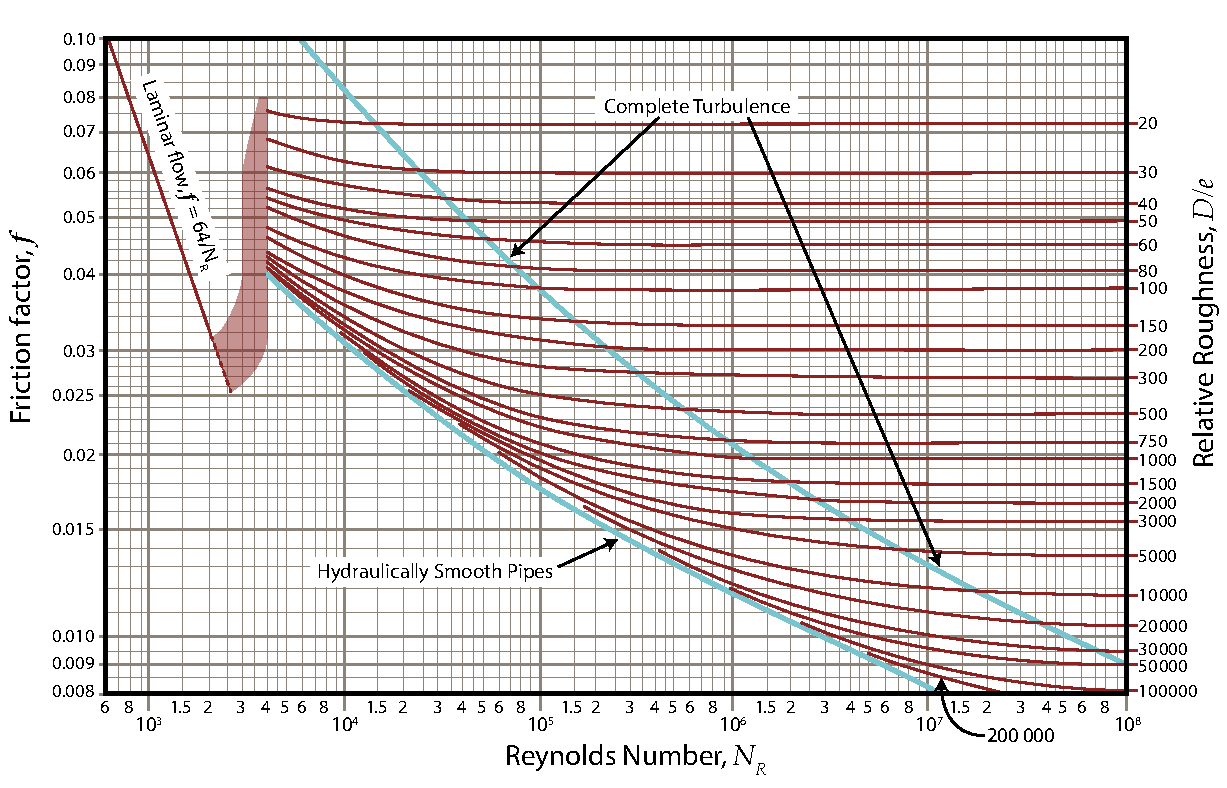
\includegraphics[scale=1.05, angle=90]{../../figs/05FrictionLosses/moody.pdf}
	\end{center}
	
	
	\newpage
	
	%%%%%%%%%%%%%%%%%%%%%%%%%%%%%%%%%%%%%%%%%%%%%%%%%%%%%%%%%%%%%%%%%%%%%%%%%%%%%%%%%%%%%%%%%%%%%%%%%%%%%%%%%%%%%%%%%%%%%
	
	\textbf{Example 4}
	Use the Moody diagram to determine the friction factor for flow with $N_R=1.6\times 10^5$ and in new clean
	$1/2$-in copper tubing.
	\parb
	(This example is done on the in-class presentation)
	
	\begin{center}
		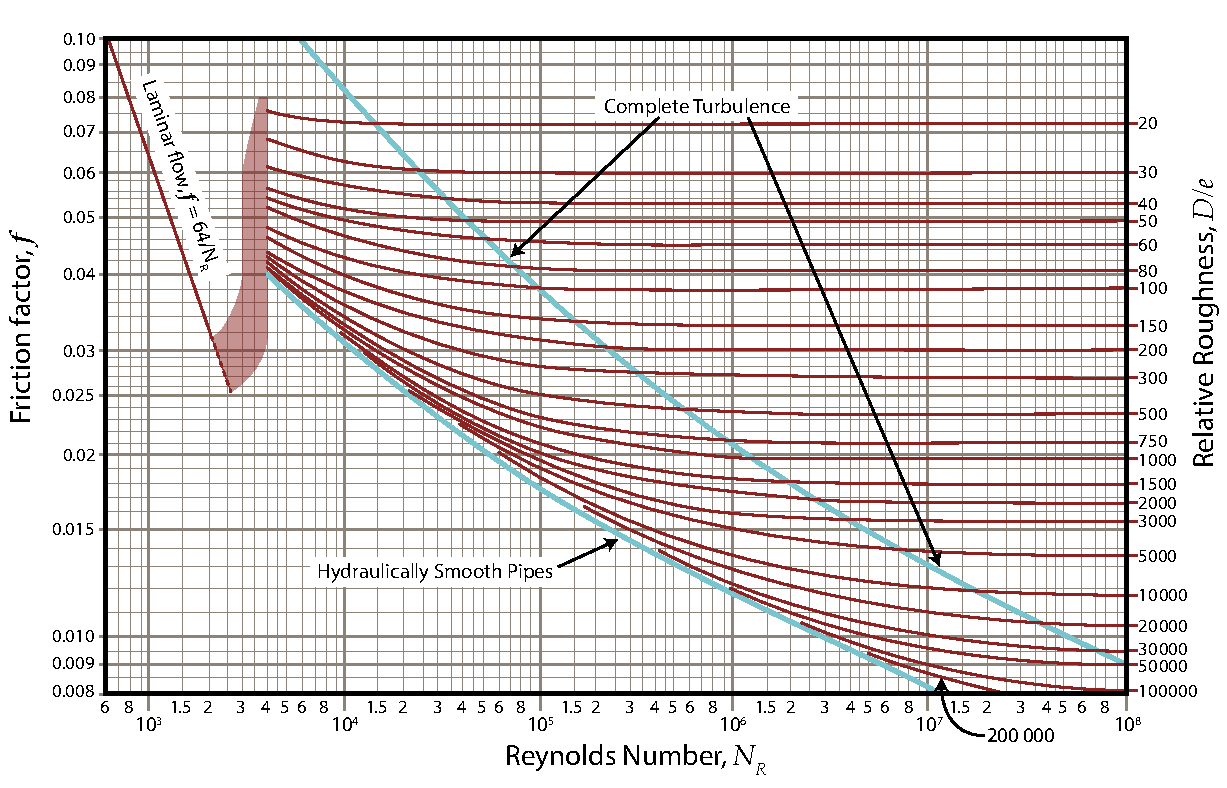
\includegraphics[scale=1.05, angle=90]{../../figs/05FrictionLosses/moody.pdf}
	\end{center}
	
	
	\newpage
	
	%%%%%%%%%%%%%%%%%%%%%%%%%%%%%%%%%%%%%%%%%%%%%%%%%%%%%%%%%%%%%%%%%%%%%%%%%%%%%%%%%%%%%%%%%%%%%%%%%%%%%%%%%%%%%%%%%%%%%
	
	\textbf{Example 5}
	A 75 m section of wooden flume is replaced with 54-in high
	density polyethylene (HDPE) pipe with inside diameter of
	1.37 m. The pipe is smooth and transports $ 190 \times 10^3\mathsf{\, m3/day}$.
	Determine the headloss due to friction in the pipe, assuming
	an average temperature of 10 \textcelsius.
	\parb
	(This example is done on the in-class presentation)
	
	\begin{center}
		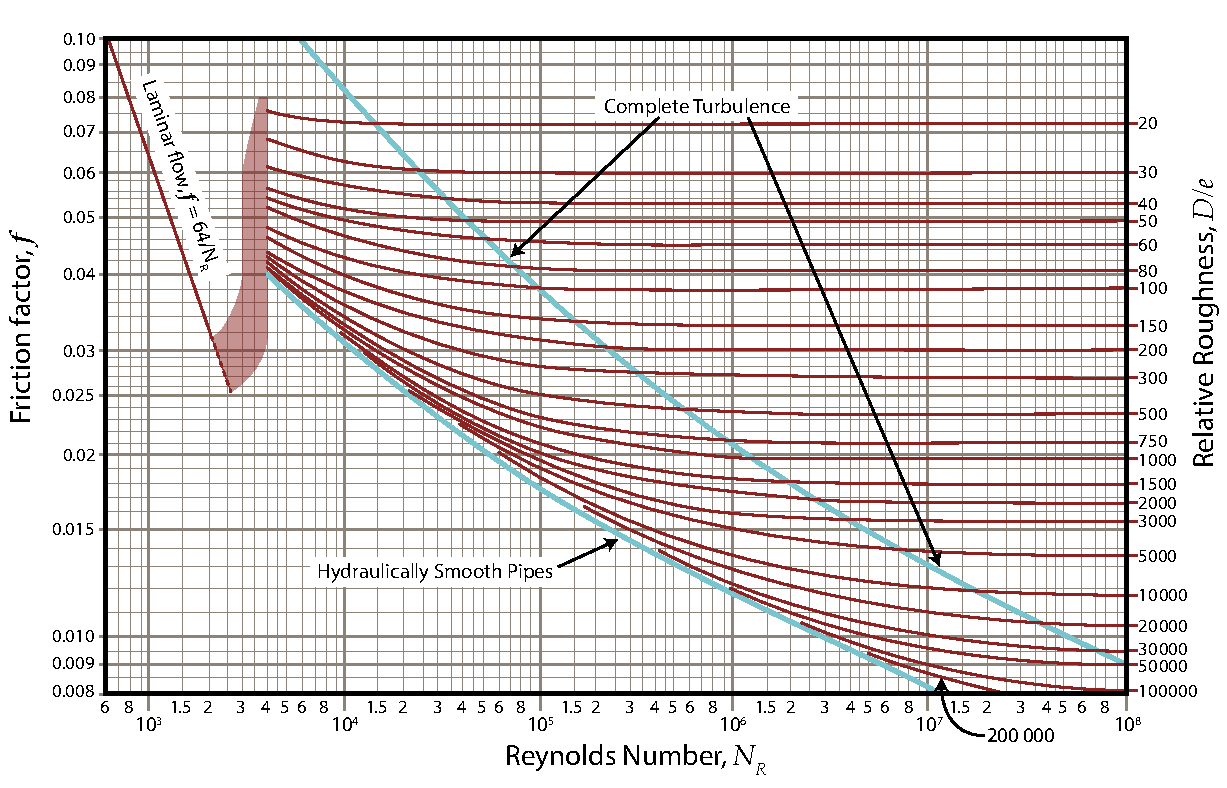
\includegraphics[scale=1.05, angle=90]{../../figs/05FrictionLosses/moody.pdf}
	\end{center}
	
	
	\newpage
	
	%%%%%%%%%%%%%%%%%%%%%%%%%%%%%%%%%%%%%%%%%%%%%%%%%%%%%%%%%%%%%%%%%%%%%%%%%%%%%%%%%%%%%%%%%%%%%%%%%%%%%%%%%%%%%%%%%%%%%
	\minit[0.475]{
		\textbf{Exercise 1}:
		
		Ethyl alcohol at $25$\textcelsius{} flows through $1\tfrac{1}{2}\text{-in}$ Schedule $80$ steel pipe at
		$5\,\text{L/s}$. Determine the pressure drop, due to friction losses, in a $125\,\text{m}$ section of pipe.
		
	}
	
	\newpage
	%%%%%%%%%%%%%%%%%%%%%%%%%%%%%%%%%%%%%%%%%%%%%%%%%%%%%%%%%%%%%%%%%%%%%%%%%%%%%%%%%%%%%%%%%%%%%%%%%%%%%%%%%%%%%%%%%%%%%
	\minit[0.5]{
		\textbf{Exercise 2}:
		\parb
		Ethyl alcohol at $25$\textcelsius{} flows through $3\text{-in}$ Schedule $80$ steel pipe at
		$5\,\text{L/s}$. Determine the pressure drop, due to friction losses, in a $125\,\text{m}$ section of pipe.
		
		
	}
	
	\newpage
	
	%%%%%%%%%%%%%%%%%%%%%%%%%%%%%%%%%%%%%%%%%%%%%%%%%%%%%%%%%%%%%%%%%%%%%%%%%%%%%%%%%%%%%%%%%%%%%%%%%%%%%%%%%%%%%%%%%%%%%
	\minit[0.5]{
		\textbf{Example 6}:
		\parb
		A horizontal $12\text{-in}$ Schedule $80$ steel pipe transports oil ($\text{sg}=0.85$,
		$\eta=3.0\times10^{-3}\;\mathsf{Pa\!\cdot\! s}$) at $185\text{ L/s}$. The pipe has pumping stations spaced at $6.0\,\text{km}$ intervals. Determine the power required by each pump to maintain the same pressure at each pump outlet if all losses are due to friction.
		
	}
	
	
	
	
	
	
	
	
	
	
	
	
	
	
\end{document}
